\documentclass{article}
\usepackage{amsmath}
\usepackage{amssymb}
\usepackage{graphicx}
\usepackage{hyperref}
\usepackage[version=4]{mhchem}


\begin{document}
\section*{Problem}
As shown in the figure, in triangle \(A B C, M\) is the midpoint of \(B C\). \(A N=\frac{1}{3} A C\). Connect \(B N\) and denote the point where \(B N\) meets \(A M\) as \(P\). Show that \(B P=3 P N\).\\
\centering
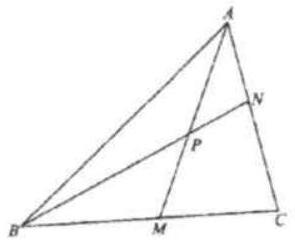
\includegraphics[width=\textwidth]{images/044.jpg}

\section*{Solution}
Method 1:\\
Take \(D\), the midpoint of \(N C\). Connect \(M D\).\\
Since \(M\) is the midpoint of \(B C, N\) is the midpoint of \(N C, M D\) \(/ / B N\) and \(M D=\frac{1}{2} B N\).\\
\centering
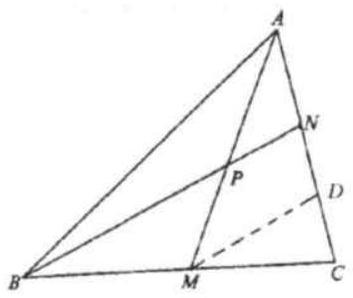
\includegraphics[width=\textwidth]{images/047.jpg}

In triangle \(C B N\), since \(M B=M C\) and \(M D / / B N, D C=D N\) and \(2 M D=B N\)

In triangle \(A M D, A N=N D=D C, P N / / M D\), so \(2 P N=M D\)

Substituting (2) into (1):\\
\(4 P N=B N \quad \Rightarrow \quad 4 P N=B P+P N \Rightarrow B P=3 P N\).

Method 2:\\
Take \(D\), the midpoint of \(B N\). Connect \(M D\).\\
Since \(M\) is the midpoint of \(B C, N\) is the midpoint of \(B N\),\\
\centering
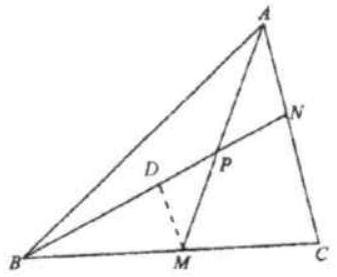
\includegraphics[width=\textwidth]{images/047(1).jpg}


\(M D / / N C\) and \(M D=\frac{1}{2} N C\).\\
In triangle \(C B N\), since \(M B=M C\) and \(M D / / C N, 2 D M=C N\) and \(D M=A N\).\\
We also see that \(\triangle A N P \sim \triangle M D P\), so \(D P=P N\).\\
\(B N=B D+D N=2 D N\)\\
\(=4 P N=3 P N+P N=B P+P N\).\\
\(\Rightarrow \quad B P=3 P N\).

\end{document}
